%%%%%%%%%%%%%%%%%%%%%%%%%%%%%%%%%%%%%%%%%%%%%%%
%%
%%  Math Thesis Template
%%  After O. Roerle, courtesy of B. Wade. Modified by Y. M. Zou on 9-10-2015.
%%  Modified by Martin G. Vieten to fit his needs.
%%
%%%%%%%%%%%%%%%%%%%%%%%%%%%%%%%%%%%%%%%%%%%%%%%
\documentclass[12pt,letterpaper,oneside,openany]{book}

% include languages for bibliography
%\usepackage[english, german, czech]{babel}

\newcommand{\name}{Jan Kretschmann}
\newcommand{\Par}{ \par \vspace{0.2cm} }
\newcommand{\pglen}{390}
\newcommand{\pts}{12pt}
\newcommand{\vs}{\vspace{0.7cm}}
\newcommand{\hs}{\hspace{5mm}}
\newcommand{\ns}{\ \Par\noindent\normalfont\normalsize\setlength{\baselineskip}{19pt}}

%\clubpenalty = 5000
%\widowpenalty = 5000

%%page settings
\usepackage[bottom=1in, top=1in, left=1in, right=1in]{geometry}
\usepackage{tikz}
%\usetikzlibrary{snakes,arrows,shapes, calc, 3d}
%\usetikzlibrary{arrows}

\usepackage{float}
\usepackage{todonotes}
\usepackage{latexsym}
\usepackage{setspace}
\usepackage{fancyhdr}
\usepackage{amsfonts}
\usepackage{amsmath}
\usepackage{mathtools}
\usepackage{amsthm}
\usepackage{amssymb}
\usepackage{mathrsfs}
\usepackage{tabularx}
\usepackage{graphicx,subfigure}
\usepackage{listings}
\usepackage{xcolor}
\usepackage{longtable}

\usepackage{layout}
\usepackage{fancyhdr}
\usepackage{setspace}
\usepackage{color}

\usepackage{cite}
%\usepackage{enumitem}
\usepackage{enumerate}

\usepackage{placeins}
%\usepackage{svjour3}
% makes counter for equation restarts for all sections
\usepackage{chngcntr}
%\usepackage[bottom=1.45in, top=1in, left=1in, right=1in]{geometry}
				
%%% Title, included  several times
\newcommand{\mytitle}{\Large \textsc{\mbox{ Master}\\
  \mbox{Thesis}}\\[20pt] \normalsize by\\
  [20pt] \name  \\[\pts] \vs }
\newenvironment{step}%
{\begin{stepp}\rm}{\rm \end{stepp}}

%% Centers the title of toc, lof and bibliography %%UWM Style
\renewcommand{\contentsname}{\begin{center}{\bf \sc  \Large Table of Contents}\end{center}}
\renewcommand{\listfigurename}{\begin{center}{\bf \sc  \Large List of Figures}\end{center}}
\renewcommand{\listtablename}{\begin{center}{\bf \sc  \Large List of Tables}\end{center}}
\renewcommand{\bibname}{\begin{center}{\bf \sc \Large Bibliography}\end{center}}



%including cleveref and changing some labels.
\usepackage[noabbrev]{cleveref}
% this will have equation references not being prefixed by ``equation''
\crefname{equation}{}{}

%this adds additional space between the labels in the lof and the captions
\makeatletter
\def\l@figure{\@dottedtocline{1}{1.5em}{3em}}
\makeatother
\makeatletter
\def\l@table{\@dottedtocline{1}{1.5em}{3em}}
\makeatother



\counterwithin{equation}{section}

\usepackage{titlesec}
\titleformat{\chapter}[display]
{\normalfont\huge\bfseries}{\thechapter.}{1em}{\Huge}
\titlespacing*{\chapter}{0pt}{50pt}{30pt} %changes free space around title of chapters


%\newtheorem{definition}{Definition}
%\newtheorem{lemma}[definition]{Lemma}
%\newtheorem{corollary}[definition]{Corollary}
%\newtheorem{example}[definition]{Example}
%\newtheorem{remark}[definition]{Remark}
%\newtheorem{theorem}[definition]{Theorem}
%\newtheorem{proposition}[definition]{Proposition}

\newtheorem{definition}[equation]{Definition}
\newtheorem{lemma}[equation]{Lemma}
\newtheorem{corollary}[equation]{Corollary}
\newtheorem{example}[equation]{Example}
\newtheorem{remark}[equation]{Remark}
\newtheorem{theorem}[equation]{Theorem}
\newtheorem{proposition}[equation]{Proposition}

\DeclareMathOperator{\Span}{span}

\definecolor{codegreen}{rgb}{0,0.6,0}
\definecolor{codegray}{rgb}{0.5,0.5,0.5}
\definecolor{codepurple}{rgb}{0.58,0,0.82}
\definecolor{backcolour}{rgb}{0.95,0.95,0.92}

\lstdefinestyle{mystyle}{
	backgroundcolor=\color{backcolour},   
	commentstyle=\color{codegreen},
	keywordstyle=\color{blue},
	numberstyle=\tiny\color{codegray},
	stringstyle=\color{red},
	basicstyle=\ttfamily\footnotesize,
	breakatwhitespace=false,         
	breaklines=true,                 
	captionpos=b,                    
	keepspaces=true,                 
	numbers=left,                    
	numbersep=5pt,                  
	showspaces=false,                
	showstringspaces=false,
	showtabs=false,                  
	tabsize=2
}

\lstset{style=mystyle}

\begin{document}
	
	\newcommand{\beqn}{\begin{displaymath}}
	\newcommand{\eeqn}{\end{displaymath}}
	\newcommand{\beqnn}{\begin{equation}}
	\newcommand{\eeqnn}{\end{equation}}
	\newcommand{\dm}{\mbox{ d}}
	\newcommand{\ginf}{\rightarrow \infty}
	\newcommand{\R}{\mathbb{R}}
	\newcommand{\N}{\mathbb{N}}
	\newcommand{\E}{\mathbb{E}}
	\newcommand{\prooff}{\noindent\textbf{Proof:} }
	\newcommand{\Bcal}{\mathscr{B}}
	\newcommand{\Dcal}{\mathscr{D}}
	\newcommand{\Pcal}{\mathcal{P}}
	\newcommand{\Qcal}{\mathscr{Q}}
	\newcommand{\Mscr}{\mathscr{M}}
	\newcommand{\Mcal}{\mathcal{M}}
	\newcommand{\Hcal}{\mathscr{H}}
	\newcommand{\Lcal}{\mathscr{L}}
	\newcommand{\Fcal}{\mathscr{F}}
	\newcommand{\Tcal}{\mathscr{T}}
	\newcommand{\beqnan}{\begin{eqnarray}}
	\newcommand{\eeqnan}{\end{eqnarray}}
	\newcommand{\beqna}{\begin{eqnarray*}}
		\newcommand{\eeqna}{\end{eqnarray*}}
	\newcommand{\prooven}{$\square$\\}
	\newcommand\restrict[1]{\raisebox{-.1ex}{$|$}_{#1}}
	\newcommand{\eps}{$\epsilon$}
	\newcommand{\pEMD}{{\mathbb{EMD}}}
	\newcommand{\cEMD}{{\mbox{EMD}_s}}
	\newcommand{\code}[1]{\texttt{#1}}
	
	\newcommand{\weightedTotal}{\mcT}
	
	
	\newcommand{\bbM}{{\mathbb{M}}}
	\newcommand{\bbD}{{\mathbb{D}}}
	\newcommand{\bbP}{{\mathbb{P}}}
	\newcommand{\bbR}{{\mathbb{R}}}
	\newcommand{\bbN}{{\mathbb{N}}}
	
	\newcommand{\V}{\mathbb{R}^n}
	
	
	\newcommand{\mcE}{{\mathcal{E}}}
	\newcommand{\mcJ}{{\mathcal{J}}}
	\newcommand{\mcP}{{\mathcal{P}}}
	\newcommand{\mcC}{{\mathcal{C}}}
	\newcommand{\mcA}{{\mathcal{A}}}
	\newcommand{\mcI}{{\mathcal{I}}}
	\newcommand{\mcR}{{\mathcal{R}}}
	\newcommand{\mcM}{{\mathcal{M}}}
	\newcommand{\mcN}{{\mathcal{N}}}
	\newcommand{\mcT}{{\mathcal{T}}}
	
	
	% this labels the chapters with capital roman literals. However, equation labels will omit
	% the roman literal when referenced in the same chapter.
	\renewcommand\theequation{\maybe{\arabic{chapter}}\arabic{section}.\arabic{equation}}
	\renewcommand{\thechapter}{\Roman{chapter}} 
	\DeclareRobustCommand\maybe[1]{\ifnum#1=\value{chapter}\relax\else\uppercase\expandafter{\romannumeral#1}.\fi}
	


\setlength{\baselineskip}{19pt}
\frontmatter




% Preliminary pages : small roman numbers
% Title Page
 \singlespace
\pagenumbering{roman}

\pagestyle{plain}
\thispagestyle{empty}
\vs\vs 
\begin{center}
	\mytitle
	\vs
	A Thesis Submitted in \\
	Partial Fulfillment of the \\
	Requirements for the Degree of \\
	\vs \vs
	\textsc{Master of Philosophy } \\ %Choose Master or PhD
	in \\
	\textsc{Mathematics} 
	\vs \vs

	at\\
	 \ \\
	The University of Wisconsin-Milwaukee\\ 
	May 2018
\end{center}

\pagebreak


%\begin{center}
%	\mytitle
%	A Thesis Submitted in \\
%	Partial Fulfillment of the \\
%	Requirements for the Degree of \\
%	 \ \\
%	\textsc{ Master of Science/Doctor of Philosophy } \\  %Choose Master or PhD
%	in \\
%	\textsc{Mathematics} \\

%	\ \\
%	at\\
%	The University of Wisconsin-Milwaukee\\ 
%	Date (Month Year) \\
%	\vs \vs
%\end{center}
%
%\thinlines \vs \vs 
%\line(1,0){\pglen} \\
%\indent  Major Professor \hspace{255pt} Date \\
%\vspace{1.3cm}\\
%\line(1,0){\pglen} \\
%\indent Graduate School Approval \hspace{200pt} Date \pagebreak

\begin{center} 
	{\large ABSTRACT} 
\end{center}
\begin{center}
	\mytitle  The University of Wisconsin-Milwaukee, 2020 \\
	Under the Supervision of Professor Jeb Willenbring 
\end{center}

\vspace{1cm}
\doublespace
\noindent Abstract


\clearpage
%\vspace*{4cm}
%\noindent Thank You.\\[2cm]
%Professor Richard Stockbridge for the invaluable guidance, advice and expertise he offered during the last four years. His support allowed me
%to fully thrive in researching and presenting this interesting topic.\\
%Professors Bruce Wade, Lei Wang, and Chao Zhu for serving on my doctoral committee and offering their feedback from reading this thesis as well
%as their insights while researching for this work.\\
%Professor Gerhard Dikta for his continued support past the Master's level, and together with Professor Martin Rei\ss el, for preparing me 
%with the right tools and skills to succeed at the doctoral level.\\[1cm]
%\begin{flushright}
%Martin G. Vieten
%\end{flushright}


\singlespace
\vspace{2cm}

%\thinlines \vs
%\noindent
%\line(1,0){\pglen} \\
%\indent  Major Professor \hspace{255pt} Date \\
\clearpage

%% Table of contents
\begin{singlespace}
\tableofcontents 
\end{singlespace}
\clearpage

\doublespace
\listoffigures
\listoftables
%% List of figures, tables, graphs, illustrations
\clearpage
\pagenumbering{arabic}

\doublespacing
\setcounter{chapter}{1}
\setcounter{section}{0}
\chapter{Introduction}
%- define earth movers distance continuous and discrete
This thesis will examine the expected value of the \emph{Earth Mover's Distance} (EMD).  To formally define the EMD, it is necessary to first define the set of joint distribution (see \cite{bourn2019expected}) :
\[
\mcJ_{\mu \nu} = \left\{ J \in \bbR^{n \times n} :
\begin{array}{l}
J \mbox{ is a non-negative real number $n$ by $n$ matrix such that } \\
\sum_{i=1}^n J_{ij} = \mu_j \mbox{ for all } j  \mbox{ and }
\sum_{j=1}^n J_{ij} = \nu_i \mbox{ for all } i
\end{array}
\right\}.
\]
where $\mcP_n$ is the set of all probability measures on a set of numbers $\{0, 1, …, n\}$ and $\mu, \nu \in \mcP_n$.
The EMD is defined as
\[
\pEMD(\mu, \nu) = \inf_{J \in \mcJ_{\mu \nu}} \sum_{i,j = 1}^n |i-j| J_{ij}.
\]
In this thesis, the practical use of the EMD will be to measure the distance between grade distributions, specifically of classes with 30 students and the grades A, B, C, D and F. Each letter grade is assigned a number by the standard \emph{Grade Point Average} (GPA): A is 4.0, B is  3.0, C is 2.0, D is 1.0 and F corresponds to 0.
In order to compute the relative distance between two grades, it is only necessary to compute the absolute value of the point grade difference: for example, the distance of a B (3.0) to a D is $|3.0-1.0|=2$ .
Some useful examples are given in \cite{bourn2019expected}: suppose there is a class with 30 students and the five grades A-F. Three possible grade distributions are given by 
\[
\begin{array}{c|ccccc}
&  A &  B &  C &  D &  F \\ \hline
X &  0 & 19 &  8 &  2 &  1 \\
Y & 12 &  2 &  5 & 11 &  0 \\
Z &  2 & 20 &  2 &  3 &  3
\end{array}
\]
Comparing distributions $X$ and $Y$, one notices they were identical if  12 A grades in $Y$ were changed to B, 5 C grades changed to B, 8 D grades  changed to C, and one D grade changed down to F. The grade movement is encoded in the matrix
\[
\left[
\begin{array}{ccccc}
0 & 0 & 0 & 0 & 0 \\
12 & 2 & 5 & 0 & 0 \\
0 & 0 & 0 & 8 & 0 \\
0 & 0 & 0 & 2 & 0 \\
0 & 0 & 0 & 1 & 0 \\
\end{array}
\right]
\]
where the columns and rows correspond to (A, B, C, D, F) and entry $(i,j)$ stands for the number of grades that were moved from position $i$ in $X$ to position $j$ in $Y$. The diagonal entries do not represent any grade change. The row sums return the $X$ distribution, while the column sums return the $Y$ distribution. The total EMD value is 26.

The grade movements between $Y$ and $Z$ are encoded in the matrix
\[
\left[
\begin{array}{ccccc}
2 & 10 & 0 & 0 & 0 \\
0 & 2 & 0 & 0 & 0 \\
0 & 5 & 0 & 0 & 0 \\
0 & 3 & 2 & 3 & 3 \\
0 & 0 & 0 & 0 & 0 \\
\end{array}
\right].
\]
also with the EMD 26, and the movements between $X$ and $Z$ are encoded in
\[
\left[
\begin{array}{ccccc}
0 & 0 & 0 & 0 & 0 \\
2 & 17 & 0 & 0 & 0 \\
0 & 3 & 2 & 3 & 0 \\
0 & 0 & 0 & 0 & 2 \\
0 & 0 & 0 & 0 & 1 \\
\end{array}
\right].
\]
with the EMD 10.
All the above distributions have the same GPA of 2.5, which shows that the EMD will distinguish between grade distributions even if the GPA is the same.
In \cite{bourn2019expected} there are three additional example distributions:
\[
\begin{array}{c|ccccc}
& A &  B & C &  D & F \\ \hline
U& 13& 13& 0& 0& 4 \\
V& 9& 1& 13& 2& 5 \\
W& 9& 7& 8& 6& 0
\end{array}
\]
this time with different GPAs, that are used to give an example for a distance matrix:
\[
\begin{array}{c|cccccc}
\text{EMD} & \text{U} & \text{V} & \text{W} & \text{X} & \text{Y} & \text{Z} \\ \hline
\text{U} & 0 & 24 & 20 & 24 & 24 & 18 \\
\text{V} & 24 & 0 & 12 & 26 & 16 & 22 \\
\text{W} & 20 & 12 & 0 & 16 & 10 & 16 \\
\text{X} & 24 & 26 & 16 & 0 & 26 & 10 \\
\text{Y} & 24 & 16 & 10 & 26 & 0 & 26 \\
\text{Z} & 18 & 22 & 16 & 10 & 26 & 0 \\
\end{array}
\]

This thesis will focus on the EMD of grade distributions with a fixed GPA. Fixing the number of students to 30 and the number of grades to 5, gives a finite number of possible distributions, which will be examined theoretically. 
Additionally, there will be an examination of real world data from the University of Wisconsin-Milwaukee. Grade distributions from the years 2014 to 2018 will be investigated, and considering only classes with 30 students and a fixed GPA allows for a comparison to the theoretical result.
At last, the classes from one year will be examined in more detail. If some grade distributions have a particularly low EMD, they will form a connected component that is persistent through a varying number of distance thresholds. These components will be visual in EMD based clustering of the grade data.


\setcounter{chapter}{2}

\chapter{Background on Formal Power Series}
\label{ch:powerseries}

\setcounter{section}{0}
\section{Generating Function for the EMD}
\label{sec:genfemd}
The approach in \cite{bourn2019expected} was to encode the distribution of the discrete EMD in the coefficients of a formal power series, which is called a \emph{generating function}.  
Let $a_0,a_1,a_2,...$ be any sequence of numbers, then the \emph{generating function} for this sequence is 
$$a_0s^0 + a_1s^1+a_2s^2+...$$
or simply $f(s)=\sum_{n=0}^{\infty}a_ns^n$. If there is an $n* \in \bbN$ such that $\forall n>n*: a_n = 0$, the series is also called \emph{generating polynomial} \cite{lando2003lectures}.
\\
The power series to encode values of the EMD is defined as
\[
H_{p,q}(z,t) := \sum_{s=0}^\infty \left( \sum_{(\mu,\nu) \in \mcC(s,p) \times \mcC(s,q)}
z^{\tiny \cEMD(\mu,\nu)} \right) t^s,
\] 
where $t$, $z$ are indeterminates and $\mcC(s,n)$ are the weak compositions of $s$ into $n$ parts, or 
\[
\mcC(s,n) = \{ (a_1, a_2, \cdots, a_n) \in \bbN^n : a_1 + \cdots + a_n = s \}.
\]
The coefficient of $t^s$  is a polynomial in $z$, which records the distribution of the discrete EMD values. 



$H_{p,q}$  is computed by:
\begin{theorem}\label{thm:HS}
	For positive integers $p$ and $q$,
	\[ H_{p,q}(z,t) = \frac{ H_{p-1,q}(z,t) + H_{p,q-1}(z,t) - H_{p-1,q-1}(z,t) }{1- z^{|p-q|} t}  \]
	if $(p,q) \neq (1,1)$ and $H_{1,1} = \frac{1}{1-t}$.
\end{theorem}
\begin{proof}
	The proof is given in \cite{bourn2019expected}.
\end{proof}


For $p=q=3$, this results in
$$H_{3, 3}(t, z)=\frac{-t^3 z^4-t^2 (2 z+1) z^2+t (z+2) z+1}{(1-t)^3 (1-t z)^2 \left(1-t z^2\right)}.$$
Expanding until $t^2$ gives the polynomial:
$$H_{3,3}(t, z)=1+t \left(2 z^2+4 z+3\right)+2 t^2 \left(z^4+2 z^3+6 z^2+6 z+3\right)+O\left(t^3\right)$$
Now, we can see that the coefficient of, for example, $t^2$ is
$$C(z)=2 z^4+4 z^3+12 z^2+12 z+6z^0$$
a polynomial in $z$. In the context of grade distributions, we are looking at 3 possible grades ($H_{3, 3}$) and classes of  2 students ($t^2$). Now, the monomials are structured as follows: $nz^k$ means, that there are $n$ possible pairs of distributions, that have an EMD of $k$. For example, there are 2 possible distributions with an EMD of 4.



Computing the weak compositions of 2, that consist of 3 elements gives us all the possible distributions in our scenario. Table \ref{tab:cs_2_3} shows a list of all the compositions.

\begin{table}
	\centering
	
	$$\begin{pmatrix}
	2 & 0 & 0 \\
	1 & 1 & 0 \\
	1 & 0 & 1 \\
	0 & 2 & 0 \\
	0 & 1 & 1 \\
	0 & 0 & 2 \\
	\end{pmatrix}$$
	
	
	\caption{Weak compositions of 2 with 3 elements.}
	\label{tab:cs_2_3}
\end{table}



In accordance with the polynomial $C$, there are only two possible pairs with an EMD of 4: $\{(2, 0, 0), (0, 0, 2)\}$ and the inverse  $\{(0,0,2),(2,0,0)\}$.

\setcounter{section}{1}
\section{Including Grade Information}
To achieve the goal of recording information on the GPA in the generating function, first define $\weightedTotal(\mu)$  as a weighted total of a distribution $\mu$ with elements $\{\mu_1, …, \mu_n\}$, specifically
$$\weightedTotal(\mu) = \sum_{i=0}^{n-1}i\mu_{i+1}$$
where $n$ is the number of elements in $\mu$. 
To include information on $\weightedTotal$, extend the power series in \cite{bourn2019expected} to:

\[
H_{p,q}(z,t, g_1, g_2) := \sum_{s=0}^\infty \left( \sum_{(\mu,\nu) \in \mcC(s,p) \times \mcC(s,q)}
g_1^{\weightedTotal(\mu)}g_2^{\weightedTotal(\nu)}z^{\tiny \cEMD(\mu,\nu)} \right) t^s,
\] 

Now, the coefficient of $t^s$ in $H_{p,q}$ is a polynomial in $z$, $g_1$ and $g_2$ whose coefficients record the distribution of  the values of $\cEMD(\mu, \nu)$, given the values of $\weightedTotal(\mu)$ and $\weightedTotal(\nu)$ saved in the exponents of $g_1$ and $g_2$.

To compute values of $H_{p,q}$, consider the following theorem \ref{thm:HSg}.

\begin{theorem}\label{thm:HSg}
 	For positive integers $p$ and $q$,
 	\[ H_{p,q}(z,t, g_1, g_2) = \frac{ H_{p-1,q}(z,t, g_1, g_2) + H_{p,q-1}(z,t, g_1, g_2) - H_{p-1,q-1}(z,tg_1, g_2) }{1- z^{|p-q|} tg_1^{p-1}g_2^{q-1}}  \]
 	if $p>1$ and $q>1$, $H_{1,1} = \frac{1}{1-t}$ and $H_{p,q}=0$ if $p<1$ or $q<1$.
\end{theorem}
\begin{proof}
	Let 
	\[
	\mcR_{p,q}^s :=  \left\{ J \in \bbM_{p,q} :(\forall i,j), J_{ij} \in \bbN, \sum_{i,j} J_{ij} = s \mbox{ and support$(J)$ is a chain}   \right\}.
	\]
	be the vector space of all degree $s$ homogeneous polynomials on $p$ by $q$ matrices, $\bbM_{p,q}$. 
 	By \cite{bourn2019expected}, we get a basis for  ($\mcR_{p,q}^s$) by considering the monomials
 	\[
 	\prod_{i=1}^p \, \, \prod_{j=1}^q x_{ij}^{J_{ij}}
 	\]
 	where $J$ is a non negative integer matrix with support on a chain.
 	
 	Assigning each monomial the expression $z^{\cEMD(\mu,\nu)} g_1^{\weightedTotal(\mu)}g_2^{\weightedTotal(\nu)}t^s$ and summing them as a formal power series, the Hilbert series is obtained:
 	\[
 	\sum_{s=0}^\infty \left( \sum_{(u,v) \in \mcC(s,p) \times \mcC(s,q)}
 	z^{\tiny \cEMD(u,v)}g_1^{\weightedTotal(u)}g_2^{\weightedTotal(v)} \right) t^s
 	\]
 	which coincides with the definition of $H_{p,q}(z, t, g_1, g_2)$. 
 	Like in \cite{bourn2019expected}, each monomial has non negative integer matrix $J$ with support on a chain as exponents. For $p$ by $q$ matrices, this chain terminates at or before $x_{p,q}^{J_{p,q}}$.
 	To factor in the cost of moving an element from position $p$ to $q$ in a distribution, the indeterminate $z$ has to be multiplied with $z^{|p-q|}$. Additionally to achieve the weighting of the totals in the exponents of $g_i$, the monomial has to be multiplied with $g_1^{p-1}g_2^{q-1}$. 
 	So in total, each monomial is multiplied with 
 	$$z^{|p-q|}g_1^{p-1}g_2^{q-1}t$$
 	and contributes $\sum_{J_{p,q}=0}^{\infty}(z^{|p-q|}g_1^{p-1}g_2^{q-1}t)^{J_{p,q}}$ to all monomials.
 	
 	Like in \cite{bourn2019expected}, $x_{pj} \subset H_{p,q-1}$ for some $1 \leq j \leq q$, and $x_{iq} \subset H_{p-1,q}$ for some $1 \leq i \leq p$. Since the exponent matrix has support on a chain, the monomials cannot be counted in both polynomials $H$.
 	
 	 %the preceding variables in the monomial contain $x_{pj}$ for some $1 \leq j \leq q$ or $x_{iq}$ for some $1 \leq i \leq p$, but not both, since the support of the exponent matrix is on a chain.
 	%The first monomial is counted in $H_{p,q-1}$ and the second in $H_{p-1,q}$. 
 	In total, the sum $H_{p,q-1}+H_{p-1,q}$ counts all monomials, but if there exists a $J_{ij}>0$ with $i<p$ and $j<q$ it is counted twice, so it has to be subtracted once by subtracting $H_{p-1, q-1}$ from the total, leaving
 	$$H_{p,q-1}+H_{p-1,q}-H_{p-1, q-1}$$
 	All monomials are counted exactly once and weighted correctly in the product:
 	\[ 
 		\frac{ H_{p-1,q}(z,t, g_1, g_2) + H_{p,q-1}(z,t, g_1, g_2) - H_{p-1,q-1}(z,tg_1, g_2) }{1- z^{|p-q|} tg_1^{p-1}g_2^{q-1}}  
 	\]
 	
 	
\end{proof}



For $p=q=3$, the adjusted formula for $H$ expanded to a series in $t$ was computed using Mathematica:
\begin{multline*}
	H_{3, 3}(z, t, g_1, g_2)=1+t ({g_1}^2 {g_2}^2+{g_1}^2 {g_2} z+{g_1}^2 z^2+{g_1} {g_2}^2 z+{g_1} {g_2}+{g_1} z+{g_2}^2 z^2+{g_2} z+1)+\\t^2 ({g_1}^4 {g_2}^4+{g_1}^4 {g_2}^3 z+2 {g_1}^4 {g_2}^2 z^2+{g_1}^4 {g_2} z^3+{g_1}^4 z^4+\\{g_1}^3 {g_2}^4 z+{g_1}^3 {g_2}^3+2 {g_1}^3 {g_2}^2 z+{g_1}^3 {g_2} z^2+{g_1}^3 z^3+2 {g_1}^2 {g_2}^4 z^2+2 {g_1}^2 {g_2}^3 z+\\2 {g_1}^2 {g_2}^2 z^2+2 {g_1}^2 {g_2}^2+2 {g_1}^2 {g_2} z+2 {g_1}^2 z^2+{g_1} {g_2}^4 z^3+{g_1} {g_2}^3 z^2+2 {g_1} {g_2}^2 z+\\{g_1} {g_2}+{g_1} z+{g_2}^4 z^4+{g_2}^3 z^3+2 {g_2}^2 z^2+{g_2} z+1)+O(t^3)
\end{multline*}


Now, the coefficient of $t^2$ contains the indeterminates $g_1$ and $g_2$ as well:
\begin{multline*}
	C(z, g_1, g_2)=g_1^4 g_2^4+g_1^4 g_2^3 z+2 g_1^4 g_2^2 z^2+g_1^4 g_2 z^3+g_1^4 z^4+g_1^3 g_2^4 z+g_1^3 g_2^3+2 g_1^3 g_2^2 z+g_1^3 g_2 z^2+ \\
	g_1^3 z^3+2 g_1^2 g_2^4 z^2+2 g_1^2 g_2^3 z+2 g_1^2 g_2^2 z^2+2 g_1^2 g_2^2+2 g_1^2 g_2 z+2 g_1^2 z^2+\\
	g_1 g_2^4 z^3+g_1 g_2^3 z^2+2 g_1 g_2^2 z+g_1 g_2+g_1 z+g_2^4 z^4+g_2^3 z^3+2 g_2^2 z^2+g_2 z+1
\end{multline*}
Each of the monomials in $C$ has the structure $ng_1^ig_2^jz^k$, which encodes the number $n$ of composition pairs with an EMD of $k$. However, in this case the compositions are restricted by $i$ and $j$, which specify the value of $\weightedTotal$ of the compositions counted. 
Specifically, $g_1^i$ means, that $\weightedTotal(\mu)=i$ must apply to the composition $\mu$ considered in the exponenet of $g_1$.

Given this information, in order to examine the EMD of compositions with a fixed value of $\weightedTotal$, the coefficient of not only $t^2$, but of $g_1^ig_2^jt^2$ has to be copmuted. Let $i=j=2$, this results again in a polynomial of $z$:
$$P(z)=2 z^2+2$$
Which means that there are 2 pairs of compositions with weighted total of  2 and a distance of 2, and there are 2 pairs of compositions with a weighted total of 0 and a distance of 0. As seen in table \ref{tab:cs_2_3}, the first monomial refers to the pairs $\{(1, 0, 1), (0, 2, 0)\}$ and $ \{(0, 2, 0), (1, 0, 1)\}$, the second monomial to the two pairs $\{(1, 0, 1), (1, 0, 1)\}$ and $\{(0, 2, 0), (0, 2, 0)\}$.


\setcounter{section}{2}
\section{Theoretical Mean EMD}

To get the theoretical average EMD of classes with 30 students, where only the grades A through F  (no +/-) are given out, the polynomial $H_{5,5}(t, z, g_1, g_2)$ has to be computed and expanded in $t$ to degree 30. Because this way of computing the polynomial requires more resources than available, the polynomial will be computed in a way similar to what was briefly shown in Section \ref{sec:genfemd}.
Instead of finding the entire polynomial $H_{5,5}(t, z, g_1, g_2)$ , the weak compositions of 30 with 5 elements were computed in Python, see Listing \ref{lst:pycomps}. From all the compositions, only those with a weighted total value $\weightedTotal$ of 90 were considered. The required polynomial in $z$ was then computed by counting the number $n$ of pairs with distance $i$, put together to the monomials $nz^i$.

%Then, extracting the coefficient of $g_1^{90}g_2^{90}t^{30}$  gives the polynomial:

\begin{multline*}
	P(z)=297z^{0}+2480z^{2}+6398z^{4}+9534z^{6}+11386z^{8}+11272z^{10}+10412z^{12}+\\8676z^{14}+7220z^{16}+5562z^{18}+4372z^{20}+3184z^{22}+2408z^{24}+\\1684z^{26}+1218z^{28}+820z^{30}+552z^{32}+348z^{34}+206z^{36}+108z^{38}+50z^{40}+18z^{42}
\end{multline*}

Examining the structure of $P(z)$, it can be seen that the coefficients of  $z$ sum up to the number of all pairs examined. Since the sum of these coefficients is the same as $P(1)$, the number of pairs can be acquired by computing that: $P(1)=$.
Additionally, since the EMD encoded in the exponent $k$ of $nz^k$ is the distance between all the $n$ distribution pairs, it follows that the coefficients $n$ of the derivative of $P$ with respect to $z$, $P'$, sum up to a total that weighs the number of pairs by the distance between each of their elements.

This implies, that to compute the average EMD between all possible distributions consisting of 30 grades that sum up to 90, it suffices to divide the weighted sum of the numbers of pairs $P'(1)$ by the total number of pairs $P(1)$, which results in:
$$\frac{P'(1)}{P(1)}=\frac{1115148}{88205} \approx 12.64268$$
To compare this result to \cite{bourn2019expected}, it is necessary to compute the unit normalized result for the mean EMD. To achieve that, the value $\frac{P'(z)}{P(z)}$ has to be divided by the maximum possible EMD. Regarding compositions of 30 with 5 elements, the highest distance is found between the distributions  $[30, 0, 0, 0, 0]$ and $[0, 0, 0, 0, 30]$, which have an EMD of 120.
Therefore, the unit normalized mean EMD of classes with 30 students and 5 grades is given by:
$$\frac{P'(z)}{120P(z)} = \frac{1115148}{120\cdot 88205} \approx 0.10536$$
The unit normalized EMD for classes of 30 students without grade restrictions has a value of 0.2191 and was computed in \cite{bourn2019expected}. 
One can see, that the theoretical mean EMD between classes of 30 students is almost exactly twice as high when there are no grade restrictions, compared to when the GPA is restricted to be a 3.0.

\todo{histogram!}


\setcounter{chapter}{3}
\chapter{Examining Grade Data}
In this chapter, the theoretical results of the mean EMD with a fixed GPA are compared to  a real world dataset, coming from the Section Attrition and Grade Report published by the Office of Assessment and Institutional Research at the University of Wisconsin-Milwaukee \cite{gradeData}. It contains the grade distributions of classes in the fall semesters from 2014 to 2018.
In the last chapter, we computed the theoretical mean EMD for grade distributions of classes with 30 students, average GPA of 3.0, where only five  grades given out, which corresponds to the letter grades A through F without plus or minus.

To compare the theoretical result to the real world data, the dataset has to be subjected to similar restrictions, without shrinking so much in size to become insubstantial.


\setcounter{section}{0}
\section{Description of Dataset}
The dataset for the fall semester of 2018 contains data from about 3300 grade distributions. Restricting the data to only classes with exactly 30 students and an exact GPA of 3.0 leaves less than 10 results, so the limitations were broadened to 25 - 35 students with a GPA between 2.9 and 3.1. 

Applying these restrictions leaves 81 classes to be further examined. 
Table \ref{tab:fall2018data} shows the first 20 entries of the data for 2018.


\begin{table}[]
	\centering
	\begin{tabular}{c||ccccccccc}
		& Cla Subject Ldesc               & Class & Enrollment & GPA   & A    & B    & C   & D   & F   \\ \hline
		0  & Music                           & 127   & 35                & 2.98  & 11 & 14 & 7 & 1 & 1 \\
		1  & Business Administration         & 335   & 30                & 347 & 12 & 9  & 3 & 3 & 1 \\
		2  & Business Administration         & 404   & 34                & 319 & 11 & 14 & 8 & 0 & 1 \\
		3  & Business Administration         & 404   & 25                & 2.987 & 6  & 13 & 5 & 0 & 0 \\
		4  & Business Administration         & 409   & 31                & 2.956 & 5  & 20 & 4 & 1 & 1 \\
		5  & Business Administration         & 409   & 34                & 2.961 & 3  & 27 & 4 & 0 & 0 \\
		6  & Business Administration         & 451   & 29                & 2.913 & 3  & 20 & 2 & 2 & 0 \\
		7  & Business Administration         & 453   & 25                & 2.988 & 11 & 9  & 2 & 2 & 1 \\
		8  & Business Administration         & 454   & 27                & 313 & 7  & 11 & 7 & 0 & 0 \\
		9  & Business Administration         & 551   & 34                & 2.921 & 11 & 12 & 8 & 3 & 0 
	\end{tabular}
	\caption{First entries of the Fall 2018 data, restricted to classes with 25-35 students and a GPA between 2.9 and 3.1}
	\label{tab:fall2018data}
\end{table}


The data was examined using Python, and the EMD of years 2014 through 2018 can be seen in table \ref{tab:emd_results}.

\begin{table}[]
	\begin{tabular}{l||llllll}
		& 2014     & 2015     & 2016     & 2017     & 2018     & Theoretical Result \\ \hline
		EMD & 16.26342 & 15.80751 & 13.18651 & 15.41643 & 16.32639 & 12.64268           \\
		Difference & 28.63902\% & 25.03289\% & 4.30152\% & 21.93955\% & 29.13709\% \\
		Unit normalized EMD & 0.08186 & 0.08014 & 0.07724 & 0.08058 & 0.07775 \\
		Classes & 79 & 63 & 84 & 77 & 72 
	\end{tabular}
	\caption{Mean EMD for the fall semesters 2014 through 2018, compared to the theoretical result}
	\label{tab:emd_results}
\end{table}

In almost all the years examined, the mean EMD is always more than 20\% higher than the theoretical result, with the largest striking differences recorded in 2014 and 2018 with EMD values that are about 28.6\% and 29.1\% larger. At least part of the difference is accounted for by the varying class sizes that had to be considered in the real world data. In the most disadvantegeous case, the difference in the number of students for a pair of classes is 10, which adds a value of at least 10 to the absolute EMD between this pair.
The only exception is the year of 2016, where the mean EMD was only 4.3\% larger than the theoretical result.

\todo{Maybe EMD comparison with curricular area, class number or whatever restricted?}

\setcounter{section}{1}
\section{Observations}
To further examine the given grade data, it can be represented as a graph, which contains each class as a vertex. Let $t$ be a threshold value for the EMD and define two vertices to be connected by an edge, if the EMD of two classes is less than or equal to $t$.

\begin{figure}
	\centering
	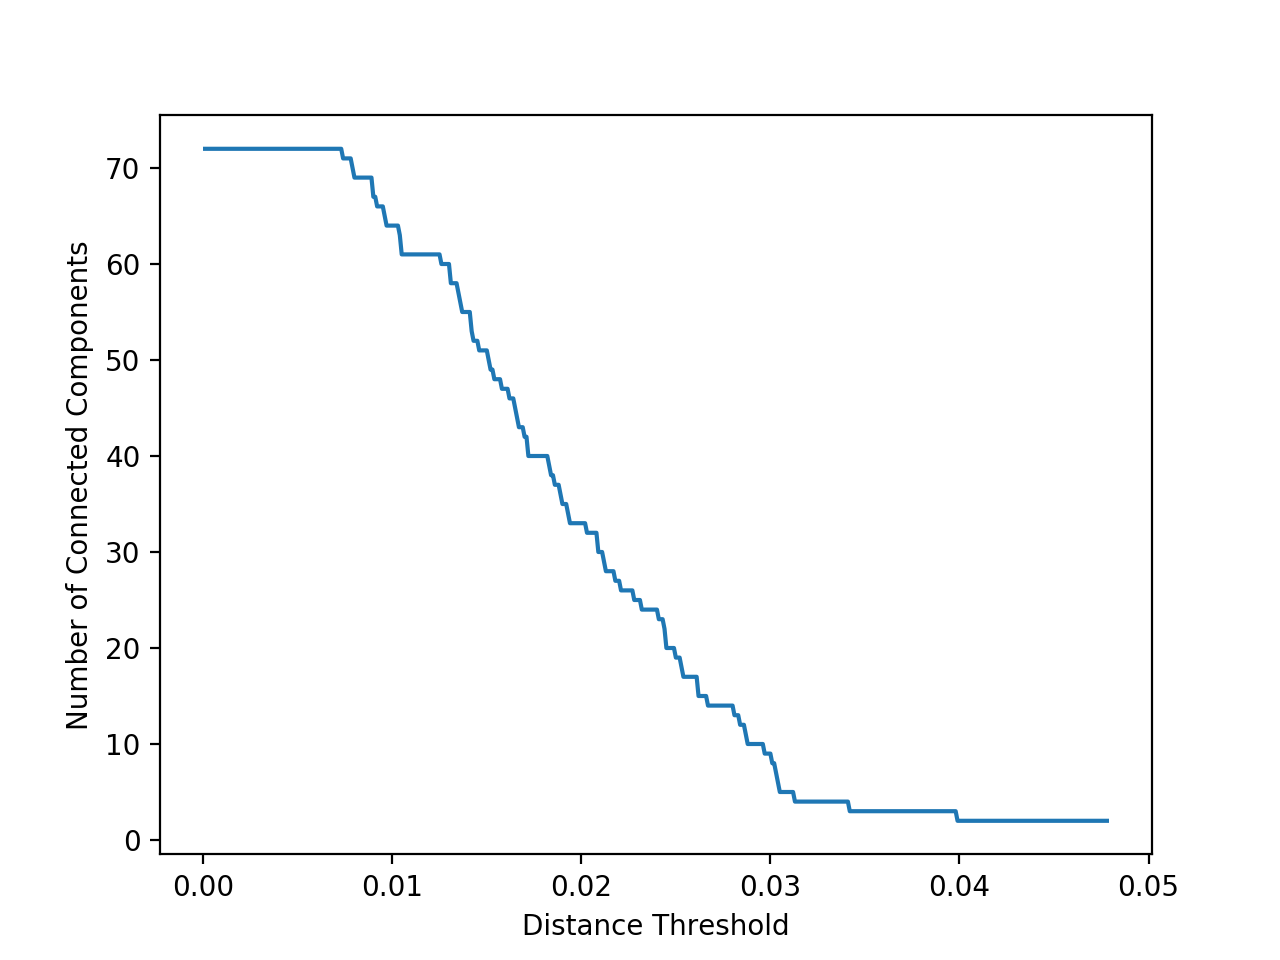
\includegraphics[width=\textwidth]{./images/n2018LLP.png}
	\caption{Distance threshold times 1000 versus number of connected components }
	\label{fig:LLP18}
\end{figure}

A connected component, per definition, is a set of vertices in a graph that are connected by a walk \cite{porter2009communities}. 
Figure \ref{fig:LLP18} refers to the dataset of Fall 2018, and shows the number of connected components as the threshold $t$ increases. With threshold $t=0$, every pair of vertices is disconnected and builds an individual connected component. As the threshold increases, there is an increasing number of edges, up to a point where the entire graph builds one connected component, at around $t=0.05$.

\begin{figure}
	\centering
	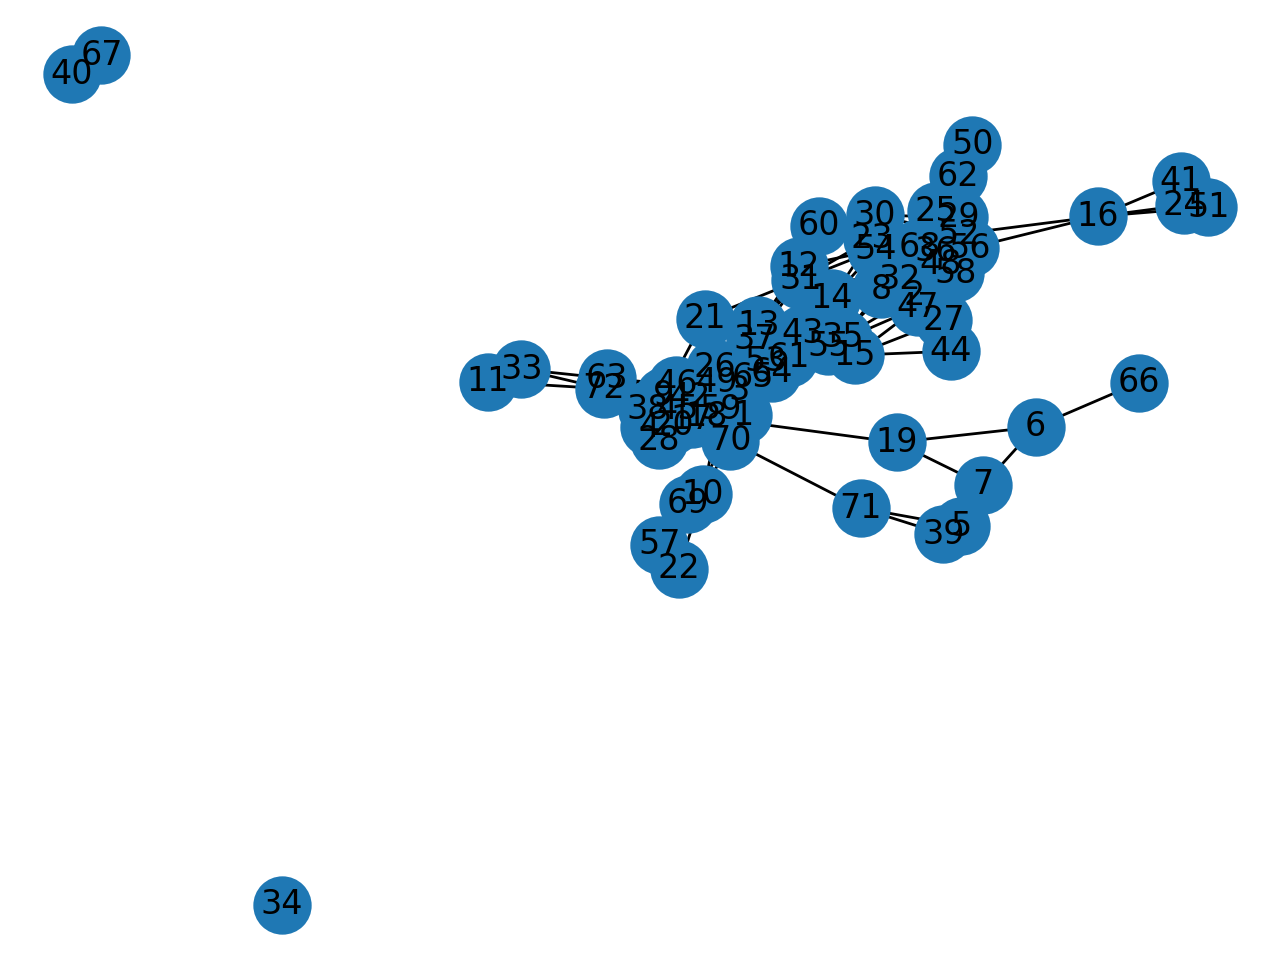
\includegraphics[width=\textwidth]{./images/n2018_th_0p035.png}
	\caption{Cluster with threshold 0.035}
	\label{fig:cluster18t035}
\end{figure}

Figure \ref{fig:cluster18t035} shows the graph when $t=0.035$, which is about half of the unit normalized mean EMD of Fall 2018, shown in table \ref{tab:emd_results}. Still, there are only 3 connected components left, with one big component containing every vertex except for $\{40, 67\}$ and $\{34\}$. For more information on the class each vertex represents, see table \ref{tab:fullfall2018} in chapter \ref{ch:appendix}.

\begin{figure}
	\centering
	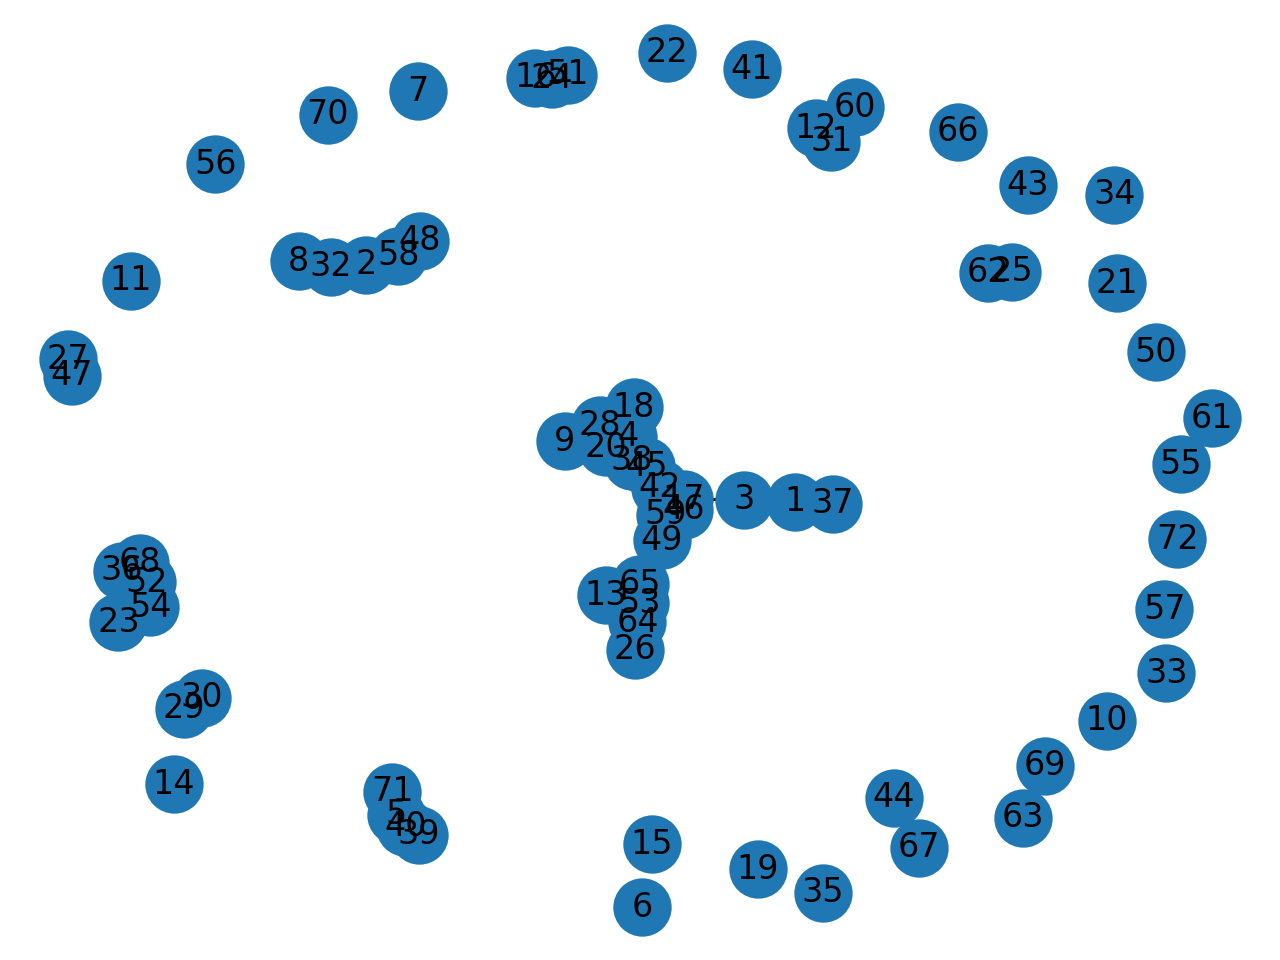
\includegraphics[width=\textwidth]{./images/n2018_th_0p0185.png}
	\caption{Cluster with threshold 0.0185}
	\label{fig:cluster18t0185}
\end{figure}

Looking at figure \ref{fig:LLP18}, there is a striking persistence in the number of connected components when $t \in [0.017, 0.0185]$. Figures \ref{fig:cluster18t0185} and \ref{fig:cluster18t017} show graphs with threshold values at boths ends of the interval, and it can be seen that some of the connected components in figure \ref{fig:cluster18t0185} are split apart in figure \ref{fig:cluster18t017}.
For instance, while $\{2, 8, 32, 58, 48\}$ form a connected component in figure \ref{fig:cluster18t0185}, they are broken apart into the components $\{2, 8, 32\}$ and $\{48, 58\}$ in figure \ref{fig:cluster18t017}.

\begin{figure}
	\centering
	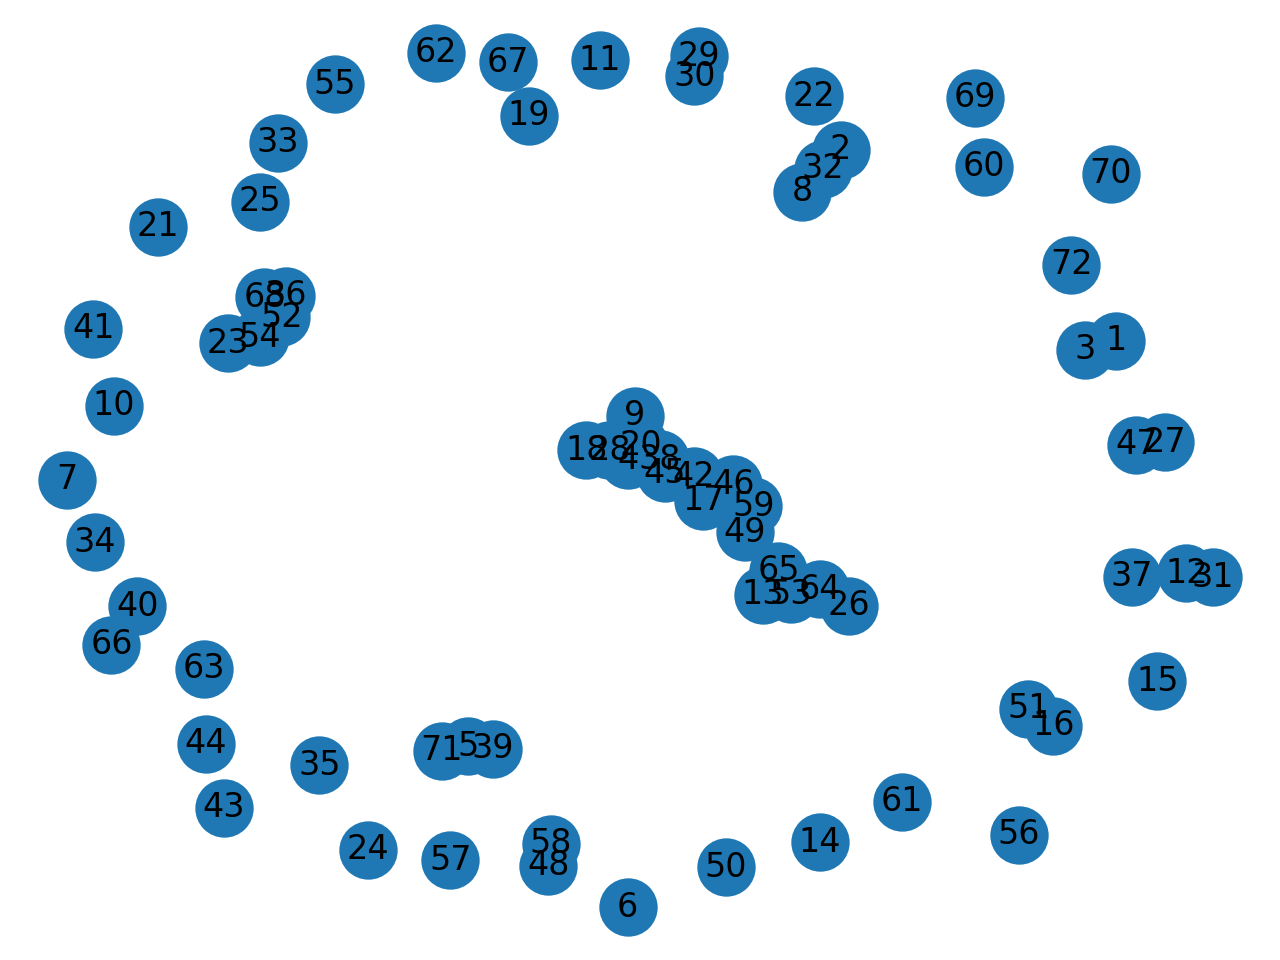
\includegraphics[width=\textwidth]{./images/n2018_th_0p017.png}
	\caption{Cluster with threshold 0.017}
	\label{fig:cluster18t017}
\end{figure}


\setcounter{chapter}{4}
\chapter{Python Code}
The dataset was examined in Python, using the library \code{pandas}. Among others, \code{pandas} includes functions to read the dataset from the given comma-separated-value (csv) format into a table, called a dataframe. \\
Dataframes  consist of  columns, that can be named with strings,  and indexed rows, as visible in table \ref{tab:fall2018data}. \code{pandas} includes Create-Read-Update-Delete (CRUD) operations for dataframes. \\
CRUD refers to the major functions of relational database management systems, and corresponding operations are also provided by the Structured Query Language (SQL, see \cite{date1993iso}) or the Hypertext Transfer Protocol (HTTP, see \cite{fielding1999hypertext}).\\
The accordance of \code{pandas} with the CRUD principles allows for efficient filtering and extracting of  relevant parts of the dataset. 
An example for these functions can be seen in listing \ref{lst:pypd}. The data set is loaded into a dataframe in line 3. \\
The first filtering operation is seen in line 6, where every row in the dataframe, that does not have a value between 25 and 35 in the column \code{Enrollment}, is removed. That is achieved by using the function \code{loc[]}, which returns a set of all rows that match the given condition, which is in this case: $|e - 30| < 5$, for all $e$ entries of the column \code{Enrollment}.
After the data is filtered for all the restrictions, it has to be brought into the format necessary for the comparison to the theoretical result from chapter 2. Only the 5 grades \code{A} to \code{F}, without plus or minus, were considered in the theoretical approach. To get the corresponding format with the given data, all the plus and minus grades were counted as their base grade. \code{pandas} supports accessing entire columns by their name, as seen in lines 9 to 11, which merge the grade columns accordingly. 
The last line of listing \ref{lst:pypd} extracts only the necessary grade columns from the data, that can then be used to calculate the EMD.


\begin{minipage}{\linewidth}
	\begin{lstlisting}[language=Python, caption={Examples for CRUD operations in Python using \code{pandas}}, label={lst:pypd}, captionpos=b]
	import pandas as pd
	
	# Load data into pandas dataframe
	data = pd.read_csv('data.csv')
	
	# Filtering for classes with 25-35 students
	data = data.loc[abs(data['Enrollment'] - 30) < 5]
	
	# Merge plus/minus grades and base grade, eg. B+, B and B- all get 
	# counted as B
	for letter in 'BCD':
	  data[letter] = data[letter+'+'] + data[letter] + data[letter+'-']
	data['A'] = data['A'] + data['A-']
	data['F'] = data['F, F+']
	
	# Extract only grade information from dataset
	data = data[['A', 'B', 'C', 'D', 'F']]
	\end{lstlisting}
\end{minipage}



\begin{minipage}{\linewidth}
	\begin{lstlisting}[language=Python, caption={Python code to compute the absolute EMD of two distributions}, label={lst:pyemd}, captionpos=b]
	def EMD(dist1, dist2):
	  dif = dist1-dist2
	  result = 0
	
	  for i in range(len(dif)):
	    # Sum difference in each iteration to account for the cost
	    # of moving an element further than one row/column
 	    result += abs(np.sum(dif[:i]))
	  return result
	\end{lstlisting}
\end{minipage}




\begin{minipage}{\linewidth}
	\begin{lstlisting}[language=Python, caption={Python code to compute the distance matrix of  a set of grade distributions, given as a pandas Series object}, label={lst:pydm}, captionpos=b]
	def build_distance_matrix(grades):
	  # Initializing an empty matrix to save the time
	  # needed to e.g. initialize everything with 0
	  distance_matrix = np.empty((len(grades), 
	    len(grades)))
	  for i in range(len(grades)):
	    # Since matrix was initialized with "random" values, 
	    # the diagonal elements have to be set to zero here
	    distance_matrix[i, i] = 0
	    for j in range(i+1, len(grades)):
	      # Distance Matrix is symmetric, so entry ij=ji
	      distance_matrix[i, j] =
	        distance_matrix[j, i] =
	        EMD(grades.iloc[i].to_numpy(
	        dtype=np.float64),
	        grades.iloc[j].to_numpy(dtype=
	        np.float64))
	  return distance_matrix
	\end{lstlisting}
\end{minipage}

\begin{minipage}{\linewidth}
	\begin{lstlisting}[language=Python, caption={Python code to compute the distance matrix of  a set of grade distributions, given as a pandas Series object.}, label={lst:pycomps}, captionpos=b]
	import scipy.special
	
	def rec_compositions(n, k, current, all_comps):
	  # Save composition if it sums to the right number
	  # and has the correct length
	  if sum(current) == n and len(current) == k:
	    all_comps.append(current)
	  # If not, start new recursive step with every possible 
	  # number appended to the composition
	  for i in range(n-sum(current)+1):
		  if len(current) < k and current not in all_comps:
		    rec_compositions(n, k, current + [i], all_comps)
    return all_comps


    def compositions(n, k):
      comps = rec_compositions(n, k, [], [])
      # The number of weak compositions of n with k elements
      # is known, so it can be checked here
      assert len(comps) == scipy.special.binom(n+k-1, k-1)
      return comps
	\end{lstlisting}
\end{minipage}




%\begin{appendices}
\clearpage
\appendix
\chapter{Appendix}
\label{ch:appendix}
 % \input{appendix/analytic-solutions}
%\end{appendices}

\begin{center}
	% Please add the following required packages to your document preamble:
	% \usepackage{longtable}
	% Note: It may be necessary to compile the document several times to get a multi-page table to line up properly
	
	\begin{longtable}{c||ccccccccc}
		\caption{Complete Fall 2018 grade dataset, restricted to classes with 25-35 students and 2.9-3.1 GPA} \\
		\label{tab:fullfall2018} 
		& Subject               & Class & Enrollment & GPA   & A    & B    & C   & D   & F   \\ \hline
		\endfirsthead
		%
		\endhead
		%
		0  & Music                           & 127   & 35                & 2.98  & 11 & 14 & 7 & 1 & 1 \\
		1  & Business Administration         & 335   & 30                & 347 & 12 & 9  & 3 & 3 & 1 \\
		2  & Business Administration         & 404   & 34                & 319 & 11 & 14 & 8 & 0 & 1 \\
		3  & Business Administration         & 404   & 25                & 2.987 & 6  & 13 & 5 & 0 & 0 \\
		4  & Business Administration         & 409   & 31                & 2.956 & 5  & 20 & 4 & 1 & 1 \\
		5  & Business Administration         & 409   & 34                & 2.961 & 3  & 27 & 4 & 0 & 0 \\
		6  & Business Administration         & 451   & 29                & 2.913 & 3  & 20 & 2 & 2 & 0 \\
		7  & Business Administration         & 453   & 25                & 2.988 & 11 & 9  & 2 & 2 & 1 \\
		8  & Business Administration         & 454   & 27                & 313 & 7  & 11 & 7 & 0 & 0 \\
		9  & Business Administration         & 551   & 34                & 2.921 & 11 & 12 & 8 & 3 & 0 \\
		10 & Business Administration         & 600   & 35                & 391 & 9  & 22 & 0 & 1 & 1 \\
		11 & Business Administration         & 703   & 25                & 2.986 & 10 & 6  & 6 & 0 & 1 \\
		12 & Business Management             & 705   & 27                & 387 & 11 & 10 & 5 & 0 & 1 \\
		13 & Curriculum and Instruction      & 112   & 30                & 387 & 12 & 9  & 4 & 1 & 1 \\
		14 & Curriculum and Instruction      & 301   & 30                & 2.954 & 10 & 13 & 3 & 1 & 2 \\
		15 & Curriculum and Instruction      & 650   & 30                & 2.953 & 15 & 5  & 4 & 1 & 3 \\
		16 & Educational Psychology          & 330   & 35                & 31  & 10 & 15 & 7 & 1 & 0 \\
		17 & Exceptional Education           & 303   & 26                & 354 & 6  & 15 & 4 & 0 & 0 \\
		18 & Exceptional Education           & 330   & 31                & 345 & 4  & 20 & 5 & 0 & 0 \\
		19 & Civil \& Envrnmntal Engineering & 456   & 26                & 338 & 7  & 13 & 6 & 0 & 0 \\
		20 & Industrial/Manufacturing Engr   & 583   & 25                & 38  & 10 & 8  & 7 & 0 & 0 \\
		21 & Mechanical Engineering          & 469   & 30                & 2.918 & 7  & 12 & 7 & 3 & 0 \\
		22 & Commun Sciences \& Disorders    & 380   & 29                & 336 & 15 & 6  & 6 & 1 & 1 \\
		23 & Kinesiology                     & 200   & 29                & 2.947 & 10 & 4  & 1 & 2 & 2 \\
		24 & Information Studies             & 310   & 35                & 359 & 16 & 12 & 2 & 1 & 3 \\
		25 & Information Studies             & 370   & 26                & 342 & 8  & 12 & 3 & 0 & 1 \\
		26 & African \& African Diaspora St  & 125   & 25                & 2.95  & 8  & 7  & 3 & 0 & 2 \\
		27 & Anthropology                    & 403   & 28                & 2.975 & 6  & 14 & 6 & 0 & 0 \\
		28 & Art History                     & 250   & 33                & 2.92  & 12 & 5  & 5 & 1 & 2 \\
		29 & Art History                     & 472   & 34                & 2.951 & 13 & 5  & 7 & 0 & 2 \\
		30 & Biological Sciences             & 529   & 28                & 34  & 11 & 7  & 6 & 0 & 1 \\
		31 & Chemistry and Biochemistry      & 341   & 33                & 311 & 14 & 10 & 4 & 3 & 1 \\
		32 & Communication                   & 101   & 27                & 3   & 6  & 13 & 1 & 1 & 1 \\
		33 & Communication                   & 363   & 25                & 397 & 10 & 7  & 4 & 0 & 0 \\
		34 & Communication                   & 410   & 25                & 2.917 & 7  & 9  & 1 & 2 & 1 \\
		35 & Economics                       & 210   & 26                & 2.937 & 13 & 7  & 3 & 1 & 2 \\
		36 & Economics                       & 325   & 35                & 2.918 & 12 & 11 & 7 & 1 & 1 \\
		37 & English                         & 205   & 26                & 354 & 7  & 13 & 5 & 0 & 0 \\
		38 & English                         & 205   & 26                & 2.903 & 4  & 16 & 2 & 1 & 1 \\
		39 & English                         & 205   & 26                & 2.957 & 14 & 4  & 0 & 0 & 5 \\
		40 & English                         & 205   & 25                & 2.914 & 12 & 6  & 1 & 1 & 3 \\
		41 & English                         & 215   & 26                & 3   & 7  & 12 & 4 & 1 & 0 \\
		42 & English                         & 215   & 25                & 344 & 9  & 10 & 2 & 1 & 1 \\
		43 & English                         & 233   & 25                & 2.954 & 8  & 9  & 2 & 0 & 3 \\
		44 & English                         & 310   & 25                & 33  & 7  & 11 & 5 & 0 & 0 \\
		45 & English                         & 517   & 25                & 2.931 & 7  & 12 & 3 & 2 & 0 \\
		46 & Food \& Beverage Studies        & 101   & 25                & 2.934 & 10 & 9  & 3 & 1 & 2 \\
		47 & Geosciences                     & 106   & 31                & 313 & 12 & 8  & 2 & 2 & 2 \\
		48 & Linguistics                     & 210   & 26                & 326 & 9  & 11 & 5 & 1 & 0 \\
		49 & Linguistics                     & 210   & 25                & 398 & 11 & 10 & 0 & 1 & 2 \\
		50 & Mathematical Sciences           & 98    & 28                & 3   & 16 & 4  & 4 & 1 & 3 \\
		51 & Mathematical Sciences           & 98    & 30                & 345 & 15 & 7  & 5 & 1 & 2 \\
		52 & Mathematical Sciences           & 98    & 29                & 336 & 10 & 12 & 4 & 1 & 1 \\
		53 & Mathematical Sciences           & 105   & 28                & 339 & 13 & 6  & 5 & 1 & 1 \\
		54 & Mathematical Sciences           & 105   & 28                & 2.936 & 9  & 10 & 4 & 2 & 1 \\
		55 & Mathematical Sciences           & 105   & 27                & 387 & 12 & 5  & 3 & 2 & 1 \\
		56 & Mathematical Sciences           & 108   & 25                & 2.933 & 9  & 7  & 6 & 3 & 0 \\
		57 & Mathematical Sciences           & 232   & 32                & 349 & 12 & 8  & 3 & 2 & 2 \\
		58 & Mathematical Sciences           & 233   & 32                & 311 & 10 & 14 & 5 & 2 & 0 \\
		59 & Philosophy                      & 101   & 29                & 359 & 11 & 5  & 6 & 1 & 0 \\
		60 & Philosophy                      & 243   & 25                & 335 & 7  & 8  & 2 & 2 & 0 \\
		61 & Philosophy                      & 250   & 30                & 317 & 10 & 8  & 1 & 0 & 2 \\
		62 & Political Science               & 361   & 33                & 311 & 8  & 17 & 2 & 3 & 0 \\
		63 & Sociology                       & 361   & 33                & 392 & 10 & 14 & 4 & 0 & 1 \\
		64 & Women's and Gender Studies      & 201   & 35                & 343 & 11 & 13 & 6 & 0 & 1 \\
		65 & Nursing                         & 673   & 28                & 348 & 5  & 21 & 2 & 0 & 0 \\
		66 & Criminal Justice                & 105   & 28                & 2.988 & 18 & 3  & 0 & 1 & 5 \\
		67 & Criminal Justice                & 460   & 32                & 2.969 & 15 & 9  & 4 & 1 & 2 \\
		68 & Criminal Justice                & 662   & 28                & 2.904 & 9  & 9  & 8 & 1 & 1 \\
		69 & Social Work                     & 753   & 31                & 2.964 & 7  & 14 & 6 & 0 & 1 \\
		70 & Architecture                    & 380   & 27                & 2.987 & 5  & 16 & 4 & 0 & 1 \\
		71 & Urban Planning                  & 316   & 28                & 343 & 7  & 14 & 2 & 1 & 0
	\end{longtable}
\end{center}



%\bibliographystyle{apalike}

\singlespace

\addcontentsline{toc}{chapter}{Bibliography}
%\renewcommand{\bibname}{Bibliography}
\bibliographystyle{alpha}
\bibliography{literature}


\end{document}
